\appendix
% \appendixpage
% \addappheadtotoc
\section{Parabola of Revolution}
\label{app:parabola}

In this section we develop the particular case of the parabola.
The parametrization is given by:

\begin{align}
x &= - \frac{1}{2}R_ct^2 + R_0 \\
y &= R_c t
\end{align}
Where $R_c$ is the radius of curvature and $R_0$ is the distance of the parabola nose to the
origin.
The respective tridimensional shape is given by:
\begin{align}
x &= -\frac{1}{2}R_ct^2 + R_0 \label{eq:x-par-a}\\
y &= R_c t \cos\phi  \label{eq:y-par-a}\\
z &= R_c t \sin\phi  \label{eq:z-par-a}
\end{align}
The azimutal angle where the surface is tangent to the line of sight in this case is given by:
\begin{align}
\sin\phi_t = -\frac{\tan i}{t} \label{eq:sin-tan-a} 
\end{align}

Subtituting (\ref{eq:sin-tan-a}) into (\ref{eq:x-par-a}), (\ref{eq:y-par-a}) and
(\ref{eq:z-par-a}) we find the apparent shape
of the paraboloid:

\begin{align}
x' &= -\frac{R_c(\frac{1}{2}t^2 \cos^2 i -\sin^2 i)}{\cos i}+R_0\cos i \\
y' &= R_c\left(t^2-\tan^2 i\right)^{1/2} 
\end{align}

Taking the limit of equations (\ref{eq:qprime}) and (\ref{eq:Aprime}) when $\theta_c$ tends to zero we find that:

\begin{align}
\left(\frac{q'}{q}\right)_{\mathrm{parabola}} &= 1+\frac{\tilde{R}_c\tan^2 i}{2}\\
\left(\tilde{R}'_c\right)_{\mathrm{parabola}} &= \frac{\tilde{R}_c}{\cos^2 i + \frac{\tilde{R}_c}{2}\sin^2 i}
\end{align}

\section{Analytic derivation of the radius of curvature in the Thin Shell model}
\label{app:rc-analytic}

For small $\theta$ we may do a polynomial expansion for the shell shape such as:

\begin{align}
R \simeq R_0\left(1+\gamma\theta^2 + \Gamma\theta^4\right) \label{eq:R-exp}
\end{align}

The radius of curvature at the axis for $R$ is given by:

\begin{align}
R_c = R_0\left(1-2\gamma\right)^{-1}
\end{align}

The coefficient gamma may be derived by an expansion at small angles of equation
(\ref{eq:th1th}), as follows:

From the first term of the right side we get:

\begin{align}
\cot\theta &\simeq \theta^{-1}\left[1-\frac{1}{3}\theta^2\right] \\
\cos^k\theta\sin^2\theta &\simeq \theta^2 - \left(\frac{1}{3} + \frac{k}{2}\right)\theta^4 \\
\implies I_k(\theta) &\simeq \frac{1}{3}\theta^3\left[ 1 - \frac{1}{10}(3k+2)\theta^2\right]\\
\implies 2\beta I_k(\theta)\cot\theta &\simeq \frac{2}{3}\beta\theta^2\left[1-\frac{1}{30}
(9k+16)\theta^2\right]\label{eq:AR1} 
\end{align}

For the second term we get:

\begin{align}
-\frac{2\beta}{k+2}\left(1-\cos^{k+2}\theta\right) & \simeq -\beta\theta^2\left[1-\frac{1}{12}
(3k+4)\theta^2\right] \label{eq:AR2}
\end{align}

For the left side we use equation (25) from \CRW{}. Then, equation (\ref{eq:th1th}) results
as follows:

\begin{align}
\theta_1^2\left(1+\frac{1}{15}\theta_1^2\right) = \beta\theta^2\left[1+\frac{1}{60}(4-9k)
\theta^2\right] \label{eq:th1th-app}
\end{align}

And we can use the approximation $\theta_1 \approx \beta\theta^2$ for the correction term in
the left side of (\ref{eq:th1th-app}):

\begin{align}
\theta_1^2 &= \beta\theta^2\left[1+\frac{1}{60}(4-9k)\theta^2\right]
\left(1-\frac{\beta}{15}\theta^2\right) \\
\implies \theta_1^2 &= \beta\theta^2\left[1+ 2C_{k\beta}\theta^2\right]
\label{eq:th1th-small}\\
\mathrm{where:~} C_{k\beta} &\equiv \frac{1}{2}\left(A_k-\frac{\beta}{15}\right) \\
A_k &\equiv \frac{1}{15}-\frac{3k}{20}
\end{align}

Now, using equation (23) from \CRW{} we may estimate $R$ at low angles. To do this, we need to
expand each term as follows (neglecting terms of order four or higher):

\begin{align}
\theta_1 = &= \beta^{1/2}\theta\left[1+ 2C_{k\beta}\theta^2\right]^{1/2} \\
\theta + \theta_1 &= \theta\left[1+\beta^{1/2}\left(1+2C_{k\beta}\theta^2\right)\right]\\
\sin\theta_1 &= \theta_1\left[1-\frac{\theta_1^2}{6}\right] \\
 &= \beta^{1/2}\theta\left[1+\left(C_{k\beta}-\frac{1}{6}\beta\right)\theta^2\right] \\
 \sin(\theta+\theta_1) &= \left[\theta+\theta_1\right]\left[1-\frac{\left(\theta+\theta_1
 \right)^2}{6}\right] \\
 &= \theta\left(1+\beta^{1/2}\right)\left\lbrace 1+\left[\frac{C_{k\beta}\beta^{1/2}}
 {1+\beta^{1/2}}-\frac{1}{6}\left(1+\beta^{1/2}\right)^2\right]\theta^2\right\rbrace
\end{align}


So, combining these terms with equation (23) from \CRW{} we found the final expression for $R$:

\begin{align}
\frac{R}{D}\equiv \frac{\sin\theta_1}{\sin(\theta+\theta_1)} = \frac{\beta^1/2}{1+\beta^{1/2}}
\left\lbrace 1 + \theta^2\left[\frac{C_{k\beta}}{1+\beta^{1/2}}+\frac{1}{6}\left(1+2\beta^{1/2}
\right)\right] \right\rbrace \label{eq:r-small-theta}
\end{align}

Returning to equation (\ref{eq:R-exp}) we see the following:

\begin{align}
R_0 &= \frac{\beta^{1/2}}{1+\beta^{1/2}} \\
\gamma &= \frac{C_{k\beta}}{1+\beta^{1/2}}+\frac{1}{6}\left(1+2\beta^{1/2}\right)
\label{eq:app-gamma}
\end{align}

We recover equation (27) of \CRW{} for $R_0$ and equation (\ref{eq:app-gamma}) is the
needed term to calculate the radius of curvature at the axis.

\section{Analytic derivation of \texorpdfstring{\boldmath $R_{90}$}{R\_90} in the thin shell model}
\label{app:r90-analytic}

To derive $R_{90}$ we need to evaluate equations (23) from \CRW{} and (\ref{eq:th1th})
at $\theta=\frac{\pi}{2}$:

\begin{align}
R_{90} = D\tan\theta_{1,90} \\
\theta_{1,90}\cot\theta_{1,90} -1 = -\frac{2\beta}{k+2} \label{eq:th190}
\end{align}
Where $\theta_{1,90}\equiv \theta_1(\frac{\pi}{2})$. Combining both equations and  introducing
the parameter $\xi\equiv \frac{2}{k+2}$ we have:
\begin{align}
R_{90} &= D\frac{\theta_{1,90}}{1-\xi\beta} \label{eq:r90-incomplete}
\end{align}

Expanding the left side of (\ref{eq:th190}) until fourth order, equation (\ref{eq:th190})
becomes:

\begin{align}
\theta_{1,90}^2\left(1+\frac{\theta_{1,90}^2}{15}\right) \simeq 3\xi\beta
\end{align}

Applying the approximation $\theta_1^2 \approx 3\xi\beta$ we found a solution
for $\theta_{1,90}$:

\begin{align}
\theta_{1,90} = \left(\frac{3\xi\beta}{1+\frac{1}{5}\xi\beta}\right)^{1/2}
\end{align}

And substituting into (\ref{eq:r90-incomplete}) we find the solution for $R_{90}$:

\begin{align}
R_{90} &= \frac{\left(3\xi\beta\right)^{1/2}}{\left(1+\frac{1}{5}\xi\beta\right)^{1/2}
\left(1-\xi\beta\right)} \\
\implies \tilde{R}_{90} &\equiv \frac{R_{90}}{R_0} = \frac{\sqrt{3\xi}\left(1+\beta^{1/2}\right)}
{\left(1+\frac{1}{5}\xi\beta\right)^{1/2}\left(1-\xi\beta\right)}
\end{align}

\section{Derivation of Characteristic Radii in Isotropic Wind/Parallel interaction Problem}
\label{app:ch-rad-Wilkin}

$\tilde{R}_{90}$ is obtained by simply evaluating equation (\ref{eq:R-Wilkin}) at $\theta=\frac{\pi}{2}$.
For the Radius of curvature we follow a similar procedure than the Wind/Wind interaction, but using equation
(\ref{eq:R-Wilkin}) for $R(\theta)$ and inserting the cosecant into the square root.

Expanding the terms of $R(\theta)$ we find the following:

\begin{align}
  \csc^2\theta &\simeq \theta^{-2}\left[1+\frac{\theta^2}{3}\left(1+\frac{\theta^2}{5}\right)\right] \\
  1-\theta\cot\theta &\simeq \frac{\theta^2}{3}\left[1 + \frac{\theta^2}{15}\left(1+\frac{2\theta^2}{21}\right)\right] \\
  \implies \tilde{R}(\theta) \simeq 1 + \frac{\theta^2}{5} + O\left[\theta^4\right]
\end{align}

From equation (\ref{eq:Rcurv}) for the radius of curvature we finally get the numerical value for $\tilde{R_c} = \frac{5}{3}$

\section{Distribution of p-values for all correlations tested}
\label{sec:distr-p-values}


\begin{figure}
  \centering
  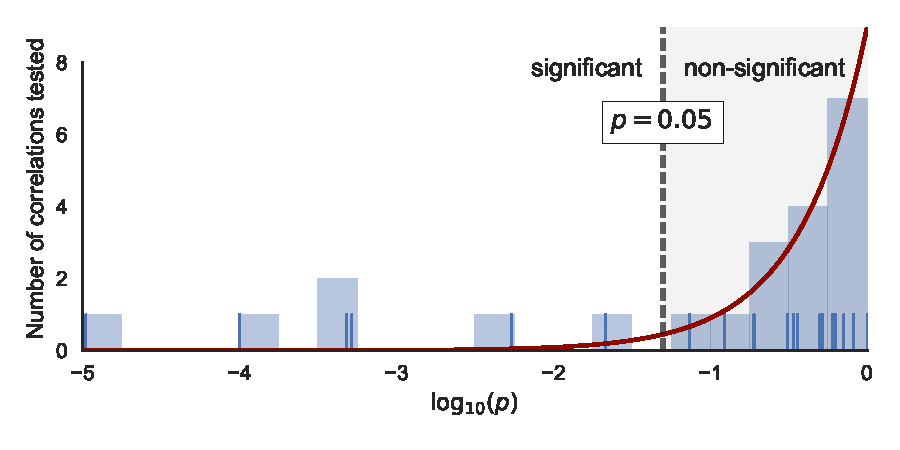
\includegraphics[width=\linewidth]{figs/p-value-histogram}
  \caption{Histogram of \(p\)-values for all Anderson--Darling
    non-parametric 2-sample tests performed during the analysis of
    section~\ref{sec:comp-with-observ}.  The vertical dashed line
    shows the traditional threshold value for significance:
    \(p = 0.05\). The red solid line shows the expected distribution
    of \(p\)-values that would be obtained if no significant
    correlations existed.}
  \label{fig:histo-p-values}
\end{figure}

All astronomical data analysis is \emph{post hoc} analysis, since the universe was not set up to test a particular hypothesis (as far as we know).  It is therefore important to guard against the ``multiple comparisons problem'', whereby seemingly significant correlations are found where none really exist, simply by virtue of the large number of tests that were carried out.

Under the more conservative Holm--Bonferroni method, only comparisons with \(p < 0.001\) would be significant. 

%%% Local Variables:
%%% mode: latex
%%% TeX-master: "quadrics-bowshock.tex"
%%% End:
